\documentclass[zihao=false,fontset=windows]{ctexart}
% ctexart 不接受任意 pt 选项。正文改 {10pt}，方括号里是行距。
\usepackage{scrextend}
\changefontsizes[12pt]{10pt}

\usepackage[a4paper,left=2.35cm,right=2.35cm,top=1.7cm,bottom=1.9cm]{geometry}
\usepackage{xcolor}
\usepackage{graphicx}
\usepackage{amsmath,amssymb}
\usepackage{enumitem}
\usepackage{tabularx}
\usepackage{colortbl}
\usepackage{listings}
\usepackage{hyperref}
\usepackage[most]{tcolorbox}

\definecolor{feishuText}{RGB}{31,35,41}
\definecolor{feishuBlue}{RGB}{36,91,219}
\definecolor{feishuRed}{RGB}{216,57,49}
\definecolor{feishuGray}{RGB}{100,106,115}
\definecolor{feishuGray2}{RGB}{143,149,158}
\definecolor{feishuPinkBg}{RGB}{251,191,188}
\definecolor{quoteBar}{RGB}{51,112,255}
\definecolor{codebg}{RGB}{245,246,247}
\definecolor{codeborder}{RGB}{222,224,227}
\definecolor{inlinebg}{RGB}{242,243,245}
\definecolor{callRed}{RGB}{253,226,226}
\definecolor{callOrange}{RGB}{255,245,235}
\definecolor{callYellow}{RGB}{254,255,240}
\definecolor{callGreen}{RGB}{240,251,239}
\definecolor{callBlue}{RGB}{240,244,255}
\definecolor{callRedSoft}{RGB}{254,241,241}
\definecolor{callSun}{RGB}{255,255,204}
\definecolor{tableHead}{RGB}{242,243,245}
\definecolor{tableRule}{RGB}{222,224,227}
\definecolor{codeText}{RGB}{31,35,41}
\definecolor{codeKeyword}{RGB}{0,0,255}
\definecolor{codeComment}{RGB}{0,128,0}
\definecolor{codeString}{RGB}{163,21,21}

\setmainfont{Times New Roman}
\setCJKmainfont{Microsoft YaHei}[AutoFakeBold=2.2]
\setCJKsansfont{Microsoft YaHei}[AutoFakeBold=2.2]
\setCJKmonofont{Microsoft YaHei}[AutoFakeBold=2.2]
\setmonofont{Consolas}
\newfontfamily\emojifont{Segoe UI Emoji}

\hypersetup{
  colorlinks=true,
  urlcolor=feishuBlue,
  linkcolor=feishuBlue,
  unicode=true,
  pdftitle={Qwen-3.5}
}

\setlength{\parindent}{0pt}
\setlength{\parskip}{0.42em}
\setlength{\fboxsep}{1.5pt}
\setlength{\emergencystretch}{3em}
\linespread{1.28}
\color{feishuText}
\arrayrulecolor{tableRule}
\urlstyle{same}

\setlist[enumerate]{label=\textcolor{feishuBlue}{\arabic*.}, leftmargin=1.7em, itemsep=0.22em, topsep=0.28em, parsep=0.08em, partopsep=0pt}
\setlist[itemize,1]{label=\textcolor{feishuBlue}{\textbullet}, leftmargin=1.35em, itemsep=0.18em, topsep=0.25em, parsep=0.06em, partopsep=0pt}
\setlist[itemize,2]{label=\textcolor{feishuBlue}{◦}, leftmargin=1.45em, itemsep=0.12em, topsep=0.15em}
\setlist[itemize,3]{label=\textcolor{feishuBlue}{\rule[0.18em]{0.38em}{0.38em}}, leftmargin=1.55em, itemsep=0.1em, topsep=0.12em}

\newcommand{\feiEmoji}[1]{{\emojifont #1}}
\newcommand{\incode}[1]{\colorbox{inlinebg}{\ttfamily\small #1}}
\newcommand{\bigmath}[1]{%
  \begin{center}\large$\displaystyle #1$\end{center}%
}

\lstset{
  language=Python,
  basicstyle=\ttfamily\footnotesize\color{codeText},
  keywordstyle=\color{codeKeyword},
  commentstyle=\color{codeComment},
  stringstyle=\color{codeString},
  showstringspaces=false,
  breaklines=true,
  columns=fullflexible,
  keepspaces=true,
  tabsize=4,
  upquote=true,
  aboveskip=2pt,
  belowskip=0pt,
  xleftmargin=0pt,
  frame=none
}

\tcbset{
  feishubase/.style 2 args={
    enhanced,
    boxrule=0pt,
    arc=8pt,
    left=10pt,
    right=10pt,
    top=7pt,
    bottom=7pt,
    before skip=6pt,
    after skip=6pt,
    colback=#1,
    colframe=#1,
    before upper={\feiEmoji{#2}\hspace{0.45em}\ignorespaces}
  }
}
\newtcolorbox{feishubox}[2]{feishubase={#1}{#2}, breakable}
\newtcolorbox{feishuboxnb}[2]{feishubase={#1}{#2}}

\newtcolorbox{feishuquote}{
  enhanced,
  breakable,
  boxrule=0pt,
  leftrule=3pt,
  arc=0pt,
  colframe=quoteBar,
  colback=white,
  left=8pt,
  right=2pt,
  top=2pt,
  bottom=2pt,
  before skip=4pt,
  after skip=4pt,
  before upper=\color{feishuGray}
}

\newtcolorbox{feishucode}{
  enhanced,
  breakable,
  colback=codebg,
  colframe=codeborder,
  boxrule=0.6pt,
  arc=6pt,
  left=6pt,
  right=6pt,
  top=5pt,
  bottom=4pt,
  before skip=6pt,
  after skip=6pt
}

\usepackage{needspace}
\definecolor{headRed}{RGB}{253,226,226}
\definecolor{headOrange}{RGB}{254,234,210}
\begin{document}
{\zihao{1}\bfseries Qwen-3.5\par}
\begin{feishuquote}来源：\href{https://scnajei2ds6y.feishu.cn/wiki/LZaXwAJi1ij54qkA2SmcGz4Fnmd}{飞书在线文档}；复刻日期：2026年10月30日。按要求省略原文代码块。\end{feishuquote}
\begin{feishubox}{callOrange}{📌}
\textbf{模型代码 PR：}\textbf{\href{https://github.com/huggingface/transformers/pull/43830/files}{transformers/pull/43830}}\par

本次开源的代码有 Qwen-3.5 和 Qwen-3.5-MOE 两类多模态大模型，本质上来说：\par

\begin{itemize}[label=\textcolor{feishuBlue}{\textbullet}]
\item \textcolor{feishuRed}{\textbf{Qwen-3.5 就是多模态版的  }}\textcolor{feishuRed}{\textbf{\href{https://my.feishu.cn/wiki/PWrdwNXobiknnlkf3uKcJLisnmb}{Qwen3 Next}}}，即把 ViT + PatchMerger 接上  \href{https://my.feishu.cn/wiki/PWrdwNXobiknnlkf3uKcJLisnmb}{Qwen3 Next}。自然地，模型也支持 Text-Only 的输出。

\end{itemize}

\begin{itemize}[label=\textcolor{feishuBlue}{\textbullet}]
\item \textcolor{feishuRed}{\textbf{Qwen-3.5-MOE 在 Qwen-3.5 基础上将 LLM Backbone 的 FFN 替换为 Qwen3 风格的 MoE}}（Top-K Router + Multi-Expert + Shared Expert），其中 Shared Expert 是 Qwen3 没有的

\end{itemize}

\end{feishubox}

\Needspace{3cm}\par\vspace{0.9em}\begin{tcolorbox}[enhanced,colback=headRed,boxrule=0pt,arc=4pt,boxsep=0pt,left=3pt,right=3pt,top=2pt,bottom=2pt,before skip=0pt,after skip=3pt]\zihao{-2}\bfseries \textcolor{feishuBlue}{1.} Qwen-3.5\end{tcolorbox}

\begin{tcbraster}[raster columns=2,raster equal height=rows,raster column skip=9pt,raster row skip=8pt]
\begin{tcolorbox}[blankest,boxrule=0pt,boxsep=0pt,left=0pt,right=0pt,top=0pt,bottom=0pt]
\begin{feishuboxnb}{callGreen}{📌}
Qwen-3.5 是一个 Dense 多模态大模型（当然也支持Text-Only模式） ：\par

\begin{itemize}[label=\textcolor{feishuBlue}{\textbullet}]
\item 多模态架构上相比\href{https://scnajei2ds6y.feishu.cn/wiki/IBFPwd8kpiW94gkOgCIcTnDZnnh}{Qwen3-VL}去除了复杂的 \incode{\href{https://scnajei2ds6y.feishu.cn/wiki/QuKwwalEei0c2hk3lN6coYC7nJd}{DeepStack}} 结构，回归了\href{https://scnajei2ds6y.feishu.cn/wiki/BHRrwQ4TAi9iCskVsMccByePngc}{Qwen2-VL}/\href{https://scnajei2ds6y.feishu.cn/wiki/S7Q2wviQhiYtQFk4jKvccQwDnWe}{Qwen2.5-VL}的 \incode{ViT + PatchMerger + LLM} 的三段式结构。

\end{itemize}

\begin{itemize}[label=\textcolor{feishuBlue}{\textbullet}]
\item LLM 架构上 Qwen-3.5 参考 \href{https://my.feishu.cn/wiki/PWrdwNXobiknnlkf3uKcJLisnmb}{Qwen3 Next} 使用支持交错 \incode{Gated/Linear Attention} 架构（每4层：3层\incode{GatedDeltaNet} + 1层\incode{Gated Attention}）

\end{itemize}

\begin{itemize}[label=\textcolor{feishuBlue}{\textbullet}]
\item 整体上看 Qwen-3.5 就是多模态版的  \href{https://my.feishu.cn/wiki/PWrdwNXobiknnlkf3uKcJLisnmb}{Qwen3 Next}。

\end{itemize}

\end{feishuboxnb}

\end{tcolorbox}
\begin{tcolorbox}[blankest,boxrule=0pt,boxsep=0pt,left=0pt,right=0pt,top=0pt,bottom=0pt]
\begin{center}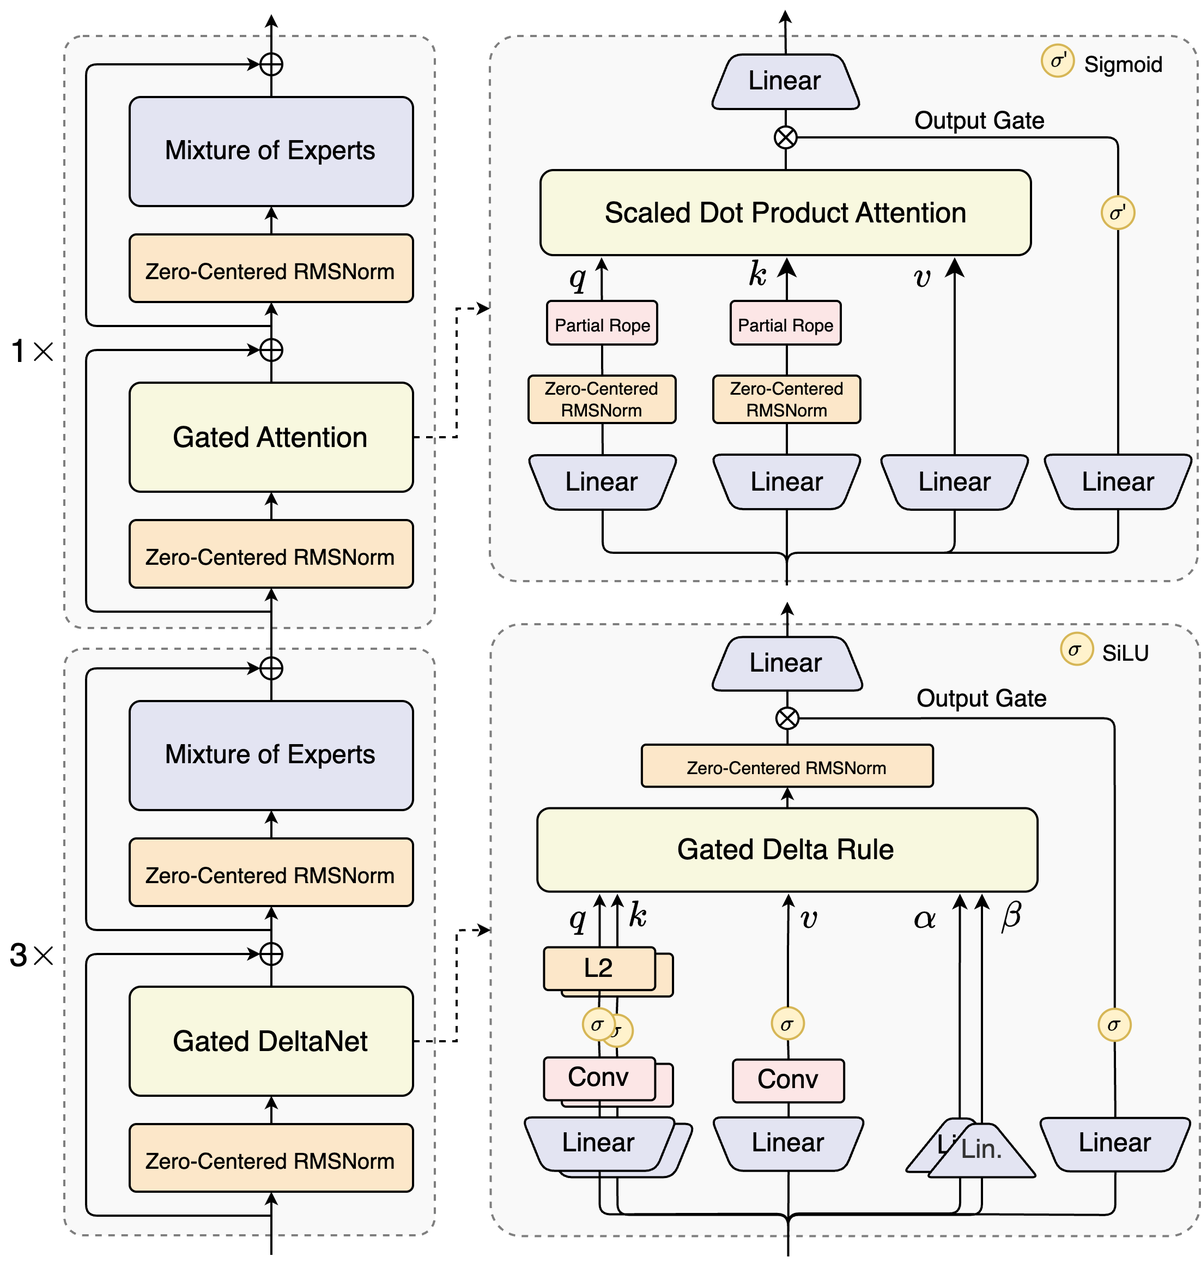
\includegraphics[width=0.98\linewidth,height=0.82\textheight,keepaspectratio]{images/Qwen-3.5/fig-01.png}\end{center}


\end{tcolorbox}
\end{tcbraster}

\Needspace{2cm}\par\vspace{0.9em}\begin{tcolorbox}[enhanced,colback=headOrange,boxrule=0pt,arc=4pt,boxsep=0pt,left=3pt,right=3pt,top=2pt,bottom=2pt,before skip=0pt,after skip=3pt]\zihao{3}\bfseries \textcolor{feishuBlue}{1.1} Vision Encoder\end{tcolorbox}

\incode{ViT} 架构回归了\href{https://scnajei2ds6y.feishu.cn/wiki/BHRrwQ4TAi9iCskVsMccByePngc}{Qwen2-VL}/\href{https://scnajei2ds6y.feishu.cn/wiki/S7Q2wviQhiYtQFk4jKvccQwDnWe}{Qwen2.5-VL} 的 \href{https://scnajei2ds6y.feishu.cn/wiki/N6PmwVkCcisDJGkC7Ypc1SfInwh}{NaViT}架构，不再使用\href{https://scnajei2ds6y.feishu.cn/wiki/IBFPwd8kpiW94gkOgCIcTnDZnnh}{Qwen3-VL}的\incode{\href{https://scnajei2ds6y.feishu.cn/wiki/QuKwwalEei0c2hk3lN6coYC7nJd}{DeepStack}} ：\par



\Needspace{2cm}\par\vspace{0.9em}\begin{tcolorbox}[enhanced,colback=headOrange,boxrule=0pt,arc=4pt,boxsep=0pt,left=3pt,right=3pt,top=2pt,bottom=2pt,before skip=0pt,after skip=3pt]\zihao{3}\bfseries \textcolor{feishuBlue}{1.2} Projector\end{tcolorbox}

Projector 沿用\href{https://scnajei2ds6y.feishu.cn/wiki/BHRrwQ4TAi9iCskVsMccByePngc}{Qwen2-VL}/\href{https://scnajei2ds6y.feishu.cn/wiki/S7Q2wviQhiYtQFk4jKvccQwDnWe}{Qwen2.5-VL}/\href{https://scnajei2ds6y.feishu.cn/wiki/IBFPwd8kpiW94gkOgCIcTnDZnnh}{Qwen3-VL}的 PatchMerger 结构：\par


在ViT内部（PatchMerger之前）维度经过切分重组，保证2x2的patch相邻：具体合并方式是通过reshape分割H，W维度之后，将两者的patch size放在num\_hidden维度的末尾。而两个merge\_size放在seq\_len的末尾，这意味着遍历reshape的时候，是2*2的patch在seq\_len维度相邻（详细可以参考\href{https://scnajei2ds6y.feishu.cn/wiki/D0tPwY7uZijRxLkQ0pDc9R0cn6g}{PatchMerger 是如何合并 2x2 的 Patch 的？}）：\par

\begin{center}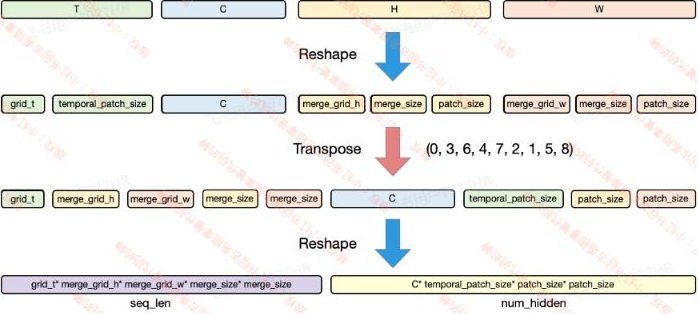
\includegraphics[width=0.85\linewidth,height=0.82\textheight,keepaspectratio]{images/Qwen-3.5/fig-02.png}\end{center}

即下图的排列方式：\par

\begin{center}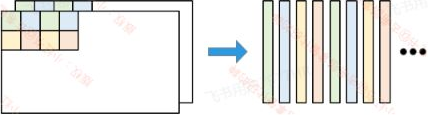
\includegraphics[width=0.52\linewidth,height=0.82\textheight,keepaspectratio]{images/Qwen-3.5/fig-03.png}\end{center}

\Needspace{11cm}\par\vspace{0.9em}\begin{tcolorbox}[enhanced,colback=headOrange,boxrule=0pt,arc=4pt,boxsep=0pt,left=3pt,right=3pt,top=2pt,bottom=2pt,before skip=0pt,after skip=3pt]\zihao{3}\bfseries \textcolor{feishuBlue}{1.3} Qwen-3.5 LLM Backbone\end{tcolorbox}

\begin{center}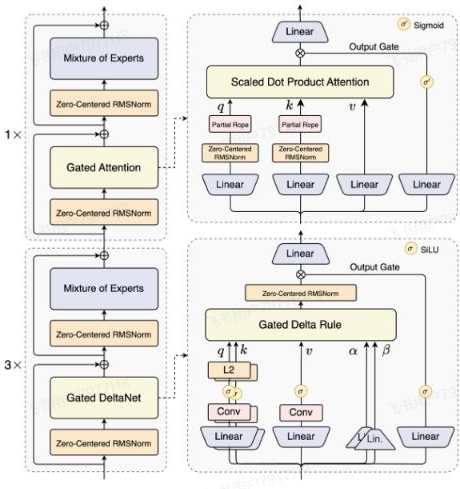
\includegraphics[width=0.56\linewidth,height=0.82\textheight,keepaspectratio]{images/Qwen-3.5/fig-04.png}\end{center}

LLM 最重要的特点是交错 \incode{Gated/Linear Attention} 架构（本质上参考的Qwen），默认是每4层Transformer Block中有3层是\incode{GatedDeltaNet} 有1层是\incode{Gated Attention}（\textcolor{feishuRed}{\textbf{比例为3:1}}），参考以下代码：\par


\Needspace{10cm}\par\vspace{0.9em}\begin{tcolorbox}[enhanced,colback=callSun,boxrule=0pt,arc=4pt,boxsep=0pt,left=3pt,right=3pt,top=2pt,bottom=2pt,before skip=0pt,after skip=3pt]\zihao{4}\bfseries \textcolor{feishuBlue}{1.3.1} \textbf{Gated Attention}\end{tcolorbox}

\begin{tcbraster}[raster columns=2,raster equal height=rows,raster column skip=9pt,raster row skip=8pt]
\begin{tcolorbox}[blankest,boxrule=0pt,boxsep=0pt,left=0pt,right=0pt,top=0pt,bottom=0pt]
首先来看Gated Attention 的两个关键特点：\par

\begin{itemize}[label=\textcolor{feishuBlue}{\textbullet}]
\item 使用了QK Norm，并且所使用的 RMSNorm 也是 Qwen3-Next 风格的 \textcolor{feishuRed}{\textbf{Zero-Centered LayerNorm。}}

\end{itemize}

\begin{itemize}[label=\textcolor{feishuBlue}{\textbullet}]
\item \incode{q\_proj} 输出维度是 *2，并显式拆出 \incode{gate}，\textcolor{feishuRed}{\textbf{输出被 learned gate 逐 token/逐 head\_dim 调制。}}

\end{itemize}

\end{tcolorbox}
\begin{tcolorbox}[blankest,boxrule=0pt,boxsep=0pt,left=0pt,right=0pt,top=0pt,bottom=0pt]
\begin{center}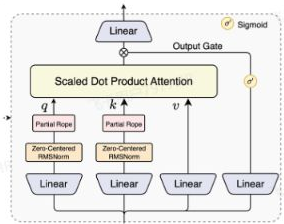
\includegraphics[width=0.98\linewidth,height=0.82\textheight,keepaspectratio]{images/Qwen-3.5/fig-05.png}\end{center}

\end{tcolorbox}
\end{tcbraster}


另外，Zero-Centered LayerNorm 代码实现如下，之所以叫Zero-Centered，是因为\incode{self.weight = }\allowbreak\incode{nn.Parameter(}\allowbreak\incode{torch.zeros(dim))}是进行0初始化的，这样一来，初始时就类似\textcolor{feishuRed}{恒等映射（scale=1）}，即标准化，不会因为 RMSNorm 未减均值造成训练不稳定：\par


对比标准RMSNorm实现：\par



\Needspace{2cm}\par\vspace{0.9em}\begin{tcolorbox}[enhanced,colback=callSun,boxrule=0pt,arc=4pt,boxsep=0pt,left=3pt,right=3pt,top=2pt,bottom=2pt,before skip=0pt,after skip=3pt]\zihao{4}\bfseries \textcolor{feishuBlue}{1.3.2} \textbf{GatedDeltaNet (Linear Attention)}\end{tcolorbox}

\begin{tcbraster}[raster columns=2,raster equal height=rows,raster column skip=9pt,raster row skip=8pt]
\begin{tcolorbox}[blankest,boxrule=0pt,boxsep=0pt,left=0pt,right=0pt,top=0pt,bottom=0pt]
Gated DeltaNet\textbf{ }用门控（gate）与可学习指数衰减（decay）把历史信息写入一个递推状态，再用查询读出。这样把原本 $O(T^2)$ 的 Softmax Attention 换成 $O(T\cdot d)$ 的递推形式，核心递推（每个 value-head，每个时刻 $t$）可写成：\par

\bigmath{\begin{aligned}s_t&=\lambda_t\odot s_{t-1}+\beta_t\odot(\Phi(k_t)\otimes v_t),\\y_t&=\Phi(q_t)\cdot s_t\end{aligned}}

其中 $0<\lambda_t<1$ 是遗忘因子（由 $g_t\leq0$ 决定，$\lambda_t=e^{g_t}),\beta_t\in(0,1)$ 是输入门，$\Phi(\cdot)$ 是对 $q,k$ 的特征映射／归一化。\par

\end{tcolorbox}
\begin{tcolorbox}[blankest,boxrule=0pt,boxsep=0pt,left=0pt,right=0pt,top=0pt,bottom=0pt]
\begin{center}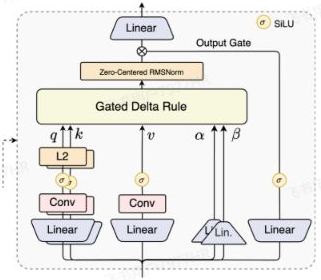
\includegraphics[width=0.98\linewidth,height=0.82\textheight,keepaspectratio]{images/Qwen-3.5/fig-06.png}\end{center}

\end{tcolorbox}
\end{tcbraster}

核心\incode{gated\_delta\_rule}代码：\par


\incode{Qwen3\_5GatedDeltaNet} 代码：\par



\Needspace{3cm}\par\vspace{0.9em}\begin{tcolorbox}[enhanced,colback=headRed,boxrule=0pt,arc=4pt,boxsep=0pt,left=3pt,right=3pt,top=2pt,bottom=2pt,before skip=0pt,after skip=3pt]\zihao{-2}\bfseries \textcolor{feishuBlue}{2.} Qwen-3.5-MoE\end{tcolorbox}

\textcolor{feishuRed}{\textbf{关键差异：}}MoE 版本把 LLM Backbone 的 FFN 从 Dense MLP 换成了 Sparse MoE（Top-K Router + Expert + Shared expert），并且额外提供 router\_logits 记录与 load-balancing aux loss 的支持，其余部分一致。\par

区别在于替换了FFN：\incode{self.mlp = Qwen3\_5MoeSparseMoeBlock(config)}\par

每个\incode{Qwen3\_5MoeSparseMoeBlock} 内部由 3 部分组成：\par

\textbf{Router（Top-K）}：\incode{Qwen3\_5MoeTopKRouter}\par
\begin{itemize}[label=\textcolor{feishuBlue}{\textbullet}]
\item \incode{router\_logits = softmax(W\_router x)}

\end{itemize}

\begin{itemize}[label=\textcolor{feishuBlue}{\textbullet}]
\item \incode{topk} 选 \incode{num\_experts\_per\_tok} 个专家

\end{itemize}

\begin{itemize}[label=\textcolor{feishuBlue}{\textbullet}]
\item \incode{router\_top\_value} 归一化作为 token 的 expert 权重

\end{itemize}


\Needspace{3cm}
\textbf{Experts（本质上是多个 FFN 权重）}：\incode{Qwen3\_5MoeExperts}\par
\begin{itemize}[label=\textcolor{feishuBlue}{\textbullet}]
\item 权重以 3D 张量存储：\incode{(num\_experts, …)}，实际执行把被路由到该 expert 的 token gather 出来跑对应 expert 的 MLP，再 scatter/index\_add 回去。

\end{itemize}


\Needspace{3cm}
\textbf{Shared Expert（共享稠密专家，本质上是必须经过的FFN，}\textcolor{feishuRed}{\textbf{但是要做gating}}\textbf{）}\par
\begin{itemize}[label=\textcolor{feishuBlue}{\textbullet}]
\item \incode{shared\_expert = Qwen3\_5MoeMLP(..., shared\_expert\_intermediate\_size)}

\end{itemize}

\begin{itemize}[label=\textcolor{feishuBlue}{\textbullet}]
\item \incode{shared\_expert\_gate = Linear(hidden, 1)}，用 \incode{sigmoid} 做 gating

\end{itemize}

\begin{itemize}[label=\textcolor{feishuBlue}{\textbullet}]
\item 最终：\incode{expert\_output += sigmoid(shared\_gate)*shared\_expert\_output}

\end{itemize}



\end{document}
